\documentclass[letterpaper]{article}
\usepackage[utf8]{inputenc}
\usepackage[parfill]{parskip}    % Activate to begin paragraphs with an empty line rather than an indent
\usepackage{graphicx}
\usepackage{amssymb}
\usepackage{amsmath}
\usepackage{amsthm}
\usepackage{mathtools}

\usepackage{afterpage}

\usepackage{algorithm}
\usepackage{algpseudocode}

\usepackage{verse}

\newtheorem{theorem}{Theorem}[section]
\newtheorem{corollary}{Corollary}[theorem]
\newtheorem{lemma}[theorem]{Lemma}

\theoremstyle{remark}
\newtheorem*{remark}{Remark}

\usepackage{epstopdf}
\usepackage{circuitikz}
\usepackage[separate-uncertainty = true,multi-part-units=single]{siunitx}
\usepackage{booktabs}
\usepackage{enumitem}
\usepackage[toc,page]{appendix}
\usepackage{color}
\usepackage{pgfplots}
\usepackage{pgfplotstable}
\usepackage{caption}
\usepackage{subcaption}
\usepackage{url}
\usepackage{multirow}
\usepackage{makecell}
\usepackage[round]{natbib}   % omit 'round' option if you prefer square brackets
\usepackage{titling}
\usepackage{siunitx}

\usepackage{setspace}
% \doublespacing
\usepackage{float}


\pgfplotsset{compat=1.14}

%  Special math symbols
%       floor, ceiling, angled brackets
%-----------------------------------------------------------------------
\newcommand{\floor}[1]{\left\lfloor #1\right\rfloor}
\newcommand{\ceil}[1]{\left\lceil #1\right\rceil}
\newcommand{\etal}{\textit{et al.}}
\newcommand{\RE}{\mathbb{R}}        % real space
\newcommand{\ZZ}{\mathbb{Z}}        % integers
\newcommand{\NN}{\mathbb{N}}        % natural numbers
\newcommand{\eps}{{\varepsilon}}    % prettier epsilon
%-----------------------------------------------------------------------
%  Tighter lists
%-----------------------------------------------------------------------
\newenvironment{itemize*}% Tighter itemized list
  {\begin{itemize}%
    \setlength{\itemsep}{-0.5ex}%
    \setlength{\parsep}{0pt}}%
  {\end{itemize}}
\newenvironment{description*}% Tighter description list
  {\begin{description}%
    \setlength{\itemsep}{-0.5ex}%
    \setlength{\parsep}{0pt}}%
  {\end{description}}
\newenvironment{enumerate*}% Tighter enumerated list
  {\begin{enumerate}%
    \setlength{\itemsep}{-0.5ex}%
    \setlength{\parsep}{0pt}}%
  {\end{enumerate}}
%-----------------------------------------------------------------------
% Typing shortcuts
%-----------------------------------------------------------------------
\newcommand{\X}{\mathbb{X}}
\newcommand{\SG}{\mathbf{S}}
\newcommand{\GE}{\mathcal{G}}
\newcommand{\ST}{\,:\,}
\renewcommand{\tilde}[1]{\widetilde{#1}}
\newcommand{\diam}{\mathrm{diam}}
\newcommand{\sq}{\square}
\newcommand{\half}[1]{\frac{#1}{2}}
\newcommand{\inv}[1]{\frac{1}{#1}}
\newcommand{\alg}{\textsf{SplitReduce}}
\newcommand{\sz}[1]{\sigma_{#1}}
\newcommand{\LL}{\mathcal{L}}
\newcommand{\softOmega}{\widetilde{\Omega}} 
\newcommand{\softO}{\widetilde{O}}
\newcommand{\OO}{O^*}  %or \widetilde{O}?

\newcommand{\norm}[1]{\left\lVert#1\right\rVert}

\newcommand{\dx}{\mathrm{d}x}
\newcommand{\dy}{\mathrm{d}y}
\newcommand{\dz}{\mathrm{d}z}
\newcommand{\dt}{\mathrm{d}t}
\newcommand{\du}{\mathrm{d}u}
\newcommand{\dtheta}{\mathrm{d}\theta}
\newcommand{\dq}{\mathrm{d}q}
\newcommand{\diff}{\mathrm{d}}
\newcommand{\dV}{\mathrm{d}V}
\newcommand{\dL}{\mathrm{d}L}
\newcommand{\dA}{\mathrm{d}A}
\newcommand{\dH}{\mathrm{d}H}
\newcommand{\df}{\mathrm{d}f}
\newcommand{\dg}{\mathrm{d}g}
\newcommand{\dr}{\mathrm{d}r}
\newcommand{\dw}{\mathrm{d}w}
\newcommand{\dv}{\mathrm{d}v}
\newcommand{\dI}{\mathrm{d}I}

\newcommand*\len[1]{\overline{#1}}

\DeclarePairedDelimiter\abs{\lvert}{\rvert}%

\newcommand\note[1]{\marginpar{\textcolor{red}{#1}}}
\newcommand*{\tageq}{\refstepcounter{equation}\tag{\theequation}}

\newcommand*{\equals}{=}

\usepackage{fancyhdr}

\pgfplotscreateplotcyclelist{grayscale}{
    thick,white!10!black,mark=x,mark options=solid, dashed\\%
    thick,white!20!black,mark=o,mark options=solid\\%
}

\newcommand{\mat}[1]{\ensuremath{\begin{bmatrix}#1\end{bmatrix}}}
\newcommand{\eqn}[1]{\begin{alignat*}{2}#1\end{alignat*}}
\newcommand{\p}[2]{\frac{\partial #1}{\partial #2}}
\newcommand*{\thus}{&\implies\quad&}

\newcommand{\answer}[1]{\framebox{$\displaystyle #1 $}}

 
\pagestyle{fancy}
\fancyhf{}
\rhead{Rahul Arya}
\lhead{EE 16B}
\cfoot{\thepage}

\title{Lecture 4 - Notes}
\author{Rahul Arya}
\date{February 2019}
\begin{document}

\maketitle

\section{Overview}
At this point, we know how to analyze circuits in two main ways: The first way, known as \emph{DC analysis}, focuses on studying the steady-state behavior of circuits with time-invariant voltage and current sources. Using the seven-step procedure from EE16A (or other faster but more specialized techniques), we can now solve for the steady-state behavior of any such circuit. The second way, known as \emph{transient analysis}, focuses on analyzing the behavior of a circuit evolving to approach its steady state. We saw this in Lecture 2, where we solved differential equations in order to characterize the behavior of MOSFETs responding to discrete changes in their input voltages. Nonetheless, in those circuits, a steady state still existed, which we could solve for.

Both in this lecture and in upcoming lectures, we will consider the ``steady-state" behavior of circuits whose sources may be continuously varying, typically in a sinusoidal manner. As the voltages and currents in these circuits almost always fail to converge to fixed values, it is difficult to understand what steady-state means in this context. We use ``steady-state" here to refer to the changing behavior of the circuit after a long period of time, after any transient effects have died off.

\section{The Inductor}
Before doing so, however, we need to add a final element to our toolbox of circuit elements - the \emph{inductor}. Broadly speaking, the inductor can be thought of as the ``dual" of the capacitor (though for our purposes this is only in a very weak sense). Whereas a capacitor stores charge, we can view an inductor as storing current. The voltage $V$ across an inductor relates to the current passing through it (using passive sign convention) like so:
\[
    V = L\frac{\dI}{\dt},
\]
where $L$ is a constant of the inductor measured in \emph{henries}. The symbol of an inductor follows:
\begin{center}
\begin{circuitikz}[american]
\draw (0, 0) to[inductor, l=$L$, v=$V$, i=$I$] (2, 0);
\end{circuitikz}
\end{center}

Inductors can be thought of as a wire of zero resistance in a particular geometry, which causes this interesting behavior. Although it is not necessary to discuss the underlying physical mechanism in detail (take Physics 5B to learn more, or look at the supplementary notes for a rushed derivation!), it's still nice to know at least intuitively what's going on. Essentially, moving charges / currents produce a magnetic field. When we vary a magnetic field, it induces an electromotive force (emf) in the current-carrying wire in the ``opposite direction" from the variation (such that a current driven by this emf would produce a magnetic field with opposite sign from the variation). However, as the emf within a perfect conductor (like the wire of an idealized inductor) must be zero, an electrostatic voltage will be produced that zeros out the net emf across the inductor. Thus, increasing the current in a wire would produce a varying magnetic field, which in turn would produce an emf opposing the current, which would induce a voltage driving the current past this emf, which would lead to a voltage drop. This voltage drop $V$ is seen in the above equation and diagram.

The constant of proportionality $L$ depends on the geometry of an inductor, and is nontrivial to compute. For a wire loop with a wire of thickness $d$ and radius $R$, the inductance $L$ is
\[
    L = \mu_0 R \ln\left(\frac{R}{d}\right),
\]
where $\mu_0$ is a physical quantity known as the \emph{permeability of free space}, and is exactly
\[
    4\pi \times 10^{-7}\SI{}{\henry \meter^{-1}}.
\]
($\mu_0$ is \emph{exactly} that value because of how the ampere is defined in relation to the meter, not because of any fundamental physical importance of the units of henries and meters).

A derivation of the inductance of a solenoid, which is a very common inductor geometry, can be found in the supplementary notes.

\section{Inductors versus Capacitors}
Now, we will try to derive the energy stored in an inductor. Imagine a voltage source $V$ placed in parallel with an inductor of inductance $L$, as shown:
\begin{center}
\begin{circuitikz}[american]
\draw (1, 1) to[inductor, l=$L$, i=$I$] (1, -1) to (0, -1) node[ground]{} to[voltage source, v=$V$, invert] (0, 1) to (1, 1);
\end{circuitikz}
\end{center}

Let the initial current $I(0) = 0$. By the equation of the inductor, we have that
\eqn{
    && V &= L\frac{\dI}{\dt} \\
    \thus \frac{\dI}{\dt} &= \frac{V}{L} \\
    \thus I(t) &= I(0) + \frac{V}{L}t \\
    &&&= \frac{V}{L}t.
}
We can calculate the energy expended by the voltage source, which is entirely stored by the inductor, to be
\eqn{
    && E_L(t) &= \int_0^t VI(t) \, \dt \\
    &&&= \frac{V^2}{L} \int_0^t t \, \dt \\
    &&&= \frac{V^2t^2}{2L} \\
    &&&= \frac{1}{2L} (I(t))^2.
}
It can be shown (try it!) that this equation holds true for all inductors, not just the inductor in this circuit. Notice how this equation is analogous to the equation for the energy in a capacitor:
\[
    E_C(t) = \frac{1}{2C} (Q(t))^2.
\]

In fact, considering the basic defining equations of capacitors and inductors, we observe similarities in the equations for current / voltage:
\eqn{
    && I &= C \frac{\dV}{\dt} \\
    && V &= L \frac{\dI}{\dt}
}
and charge / magnetic flux:
\eqn{
    && Q &= CV \\
    && \phi &= LI.
}
(By the way, if you're wondering about that $\phi$ describing the magnetic flux, read the supplementary notes to find out more. But I don't think it's necessary for this course.)

These similarities can also be seen visually. Consider a current source $I(t)$ placed in series with a capacitor $C$:
\begin{center}
\begin{circuitikz}[american]
\draw (2, 1) to[capacitor, v=$V$, l=$C$] (2, -1) to (0, -1) node[ground]{} to[current source, i^>=$I$] (0, 1) to (2, 1);
\end{circuitikz}
\end{center}
Plotting the varying voltage $V(t)$ across the capacitor against the supplied current $I(t)$, we can easily determine:
\begin{center}
\begin{tikzpicture}
\begin{axis}[
    xmin=0, xmax=5,
    ymin=-1.5, ymax=2.5,
    axis lines=middle, xtick=\empty, ytick=\empty,
    xlabel=$t$,
]
\addplot [mark=none, dashed] coordinates {(0, 0) (1, 0) (1, 2) (2, 2) (2, 0) (3, 0) (3, -1) (4, -1) (4, 0) (5, 0)};
\addplot [mark=none] coordinates {(0, 0) (1, 0) (2, 2) (3, 2) (4, 1) (5, 1)};
\addlegendentry{$I(t)$}
\addlegendentry{$V(t)$}
\end{axis}
\end{tikzpicture}
\end{center}

Now, consider a varying voltage source $V(t)$ placed in series with an inductor $L$:
\begin{center}
\begin{circuitikz}[american]
\draw (2, 1) to[inductor, i=$I$, l=$L$] (2, -1) to (0, -1) node[ground]{} to[voltage source, v=$V$, invert] (0, 1) to (2, 1);
\end{circuitikz}
\end{center}
Plotting the varying current $V(t)$ through the inductor against the supplied voltage $I(t)$ across the capacitor, we can easily determine:
\begin{center}
\begin{tikzpicture}
\begin{axis}[
    xmin=0, xmax=5,
    ymin=-1.5, ymax=2.5,
    axis lines=middle, xtick=\empty, ytick=\empty,
    xlabel=$t$,
]
\addplot [mark=none, dashed] coordinates {(0, 0) (1, 0) (1, 2) (2, 2) (2, 0) (3, 0) (3, -1) (4, -1) (4, 0) (5, 0)};
\addplot [mark=none] coordinates {(0, 0) (1, 0) (2, 2) (3, 2) (4, 1) (5, 1)};
\addlegendentry{$V(t)$}
\addlegendentry{$I(t)$}
\end{axis}
\end{tikzpicture}
\end{center}
Note that both axes use arbitrary units.

Observe that these two graphs look remarkably similar. This is not a coincidence, and again reflects the similarities between inductors and capacitors.

\section{Impedance}
Now, we will begin to consider sinusoidal voltage and current sources. Consider the voltage source $V(t) = V_0\sin{\omega t}$. Note that $\omega$ represents the \emph{angular velocity} of the supply, and has units of \SI{}{\radian / \second}. We will place this voltage source in series with a capacitor $C$, as shown:
\begin{center}
\begin{circuitikz}[american]
\draw (2, 1) to[capacitor, i=$I$, l=$C$] (2, -1) to (0, -1) node[ground]{} to[sinusoidal voltage source, v<=$V(t)$] (0, 1) to (2, 1);
\end{circuitikz}
\end{center}

By the capacitor equation, we have that
\eqn{
    && I &= C \frac{\dV}{\dt} \\
    &&&= \omega C V_0 \cos{\omega t}.
}
Thus, we see that the current through the capacitor is 90 degrees ahead of the voltage supplied. For now, however, we will disregard the phases of the signals, and focus instead on their amplitudes. 

We define the \emph{impedance} $Z$ to be a quantity whose magnitude $\abs{Z}$ is
\[
    \abs{Z} = \frac{\abs{V}}{\abs{I}},
\]
where $\abs{V}$ and $\abs{I}$ are the amplitudes of the voltage and current signals, respectively. We will see in future lectures that $Z$ is really a complex number whose argument represents the phase offset of the voltage signal with respect to the current, but this fact can be disregarded for now. Instead, imagine $\abs{Z}$ simply as a quantity analogous to that of resistance from DC circuit analysis, which also has units of ohms.

Computing the impedance of the capacitor, we obtain
\[
    \abs{Z_C} = \frac{1}{\omega C},
\]
indicating that the capacitor resists the voltage signal (and allows a smaller current to flow back and forth) when $\omega$ is small, and the voltage source oscillates less rapidly. In particular, note that a DC voltage source can be thought of as having $\omega = 0$ (this is not strictly correct, since then $V(t) = 0$, but we can view $V(t) = V_0\cos{\omega t}$ for the calculations to work out right), which would lead to the capacitor having an infinite impedance. This makes sense, since DC current cannot steadily flow through a capacitor indefinitely.

Now, we will look at the equivalent circuit for inductors, with a sinusoidal current source $I(t) = I_0\sin{\omega t}$ placed in series with an inductor $L$, as shown:
\begin{center}
\begin{circuitikz}[american]
\draw (2, 1) to[inductor, v=$V$, l=$L$] (2, -1) to (0, -1) node[ground]{} to[sinusoidal current source, i=$I(t)$] (0, 1) to (2, 1);
\end{circuitikz}
\end{center}

Applying the equation for an inductor, we obtain
\eqn{
    && V &= L \frac{\dI}{\dt} \\
    &&&= \omega L I_0 \cos{\omega t} \\
    \thus \abs{Z_L} &= \omega L,
}
computing the magnitude of the impedance $\abs{Z_L}$ in a similar manner to before.

Observe that when we supply DC current ($\omega = 0$), $\abs{Z_L} = 0$, suggesting that the inductor behaves like a short. This makes sense, since the interesting properties of an inductor only have an effect when the supply is varying; otherwise, an inductor behaves just like the ideal wire that it is composed of.

Let's try out some real values for capacitance and inductance, to get an idea for what these equations mean. We will let $C = \SI{1}{\pico\farad}$ and $L = \SI{1}{\nano\henry}$, which are reasonably realistic values for these components. We will consider two possible frequencies: $f = \SI{60}{\hertz}$ (like that provided from the mains AC power\footnote{At least when the power company isn't burning down half the state.}), and, at the other end of the spectrum, $f = \SI{3}{\giga\hertz}$ (of the order of the clock rate of a modern CPU).

If we have some frequency $f$ describing the rotation of some angular quantity, then the quantity rotates $2\pi$ radians every cycle, or $2\pi f$ radians per second. Thus, we can write the angular velocity $\omega$ as
\[
    \omega = 2\pi f,
\]
for substitution into our results for impedance.

Considering the capacitor, we obtain
\eqn{
    && \abs{Z_C(f = \SI{60}{\hertz})} &= \SI{2.5}{\giga\ohm} \\
    && \abs{Z_C(f = \SI{3}{\giga\hertz})} &= \SI{50}{\ohm}.
}
As can be seen, the capacitor has an extremely high resistance at low frequencies, as we expected. In fact, resistances / impedances in the gigaohm range can be comfortably treated as open circuits for most practical purposes. In contrast, at high frequencies, the capacitor allows non-negligible currents to pass through. Therefore, we can think of a capacitor as acting as a filter that only allows high frequencies to pass through, commonly referred to as a \emph{high-pass filter}. 

This is because at lower frequencies, current flows in one direction for longer, ``filling up" the capacitor to a greater extent, reducing the flow of charge and making the capacitor behave more like an open circuit, whereas at high frequencies, the capacitor never has a chance to fill up enough before the voltage polarity flips. 

Now, considering the inductor, we similarly obtain
\eqn{
    && \abs{Z_L(f = \SI{60}{\hertz})} &= \SI{0.4}{\micro\ohm} \\
    && \abs{Z_L(f = \SI{3}{\giga\hertz})} &= \SI{20}{\ohm}.
}
Here, we see the reverse phenomenon - practically zero resistance at low frequencies, and non-negligible resistance at higher frequencies, again as we expected. Therefore, we can think of an inductor as acting as a filter that only allows low frequencies to pass through, commonly referred to as a \emph{low-pass filter}. 

This is because at high frequencies the magnetic field of the inductor is flipping back and forth rapidly, producing a large negative emf that induces a large voltage drop, whereas at lower frequencies the magnetic field has less of an impact, making the inductor behave more like a short.

\section{Frequency Response Magnitude Plots}
Now, we will explore an intuitive way of visualizing the frequency response of slightly more complex circuits to AC current and voltage sources. Modern devices often operate at a wide range of frequencies, from the \SI{60}{\hertz} of our mains power, to the \SI{100}{\mega\hertz} of radio, to almost \SI{100}{\giga\hertz} in cutting-edge wireless transmission standards - almost $10$ orders of magnitude. 

This huge variation in frequency leads to a corresponding variation in impedance. Thus, when plotting impedance against frequency, we will use a log-log plot, to make these immense orders of magnitude more tractable. From our previous results, we have that
\eqn{
    && \abs{Z_C} &= \frac{1}{\omega C} \\
    \thus \log{\abs{Z_C}} &= -\log{C} - \log{\omega}
}
and
\eqn{
    && \abs{Z_L} &= \omega L \\
    \thus \log{\abs{Z_L}} &= \log{L} + \log{\omega}.
}
Thus, our log-log plot will be entirely linear. Plotting a capacitor $C = \SI{1}{\pico\farad}$ and an inductor $L = \SI{1}{\henry}$, as well as a resistor $\abs{Z_R} = R = \SI{1}{\ohm}$, we obtain:
\begin{center}
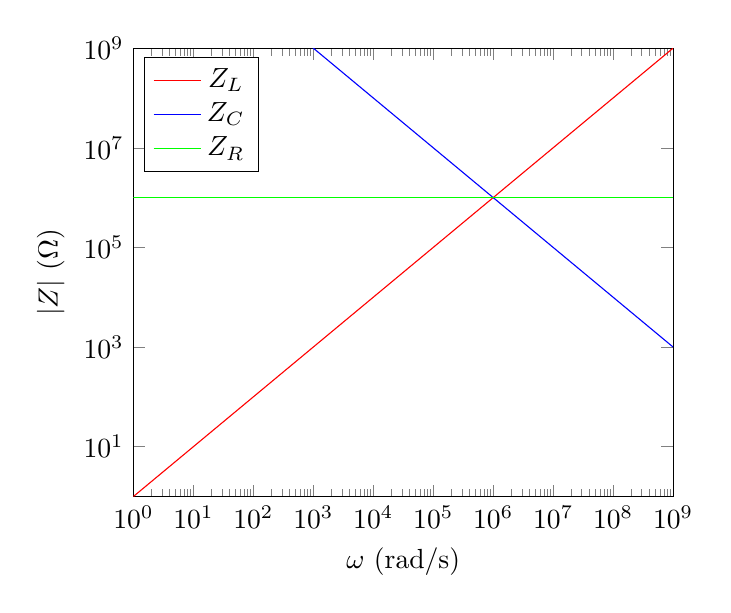
\begin{tikzpicture}
\begin{loglogaxis}[
    xlabel=$\omega$ (\SI{}{\radian / \second}), ylabel=$\abs{Z}$ (\SI{}{\ohm}),
    xmin=1, xmax=10^9,
    ymin=1, ymax=10^9,
    legend style={at={(0.02,0.98)},anchor=north west},
 ]
\addplot [domain=1:1000000000, color=red] {x};
\addplot [domain=1:1000000000, color=blue] {10^12 / x};
\addplot [domain=1:1000000000, color=green] {10^6};
\addlegendentry{$Z_L$}
\addlegendentry{$Z_C$}
\addlegendentry{$Z_R$}
\end{loglogaxis}
\end{tikzpicture}
\end{center}
From our previous algebraic calculations, we see that an increase in inductance will increase an inductor's impedance, while an increase in capacitance will decrease a capacitor's impedance. The nature of capacitors and inductors as high- and low-pass filters, respectively, is also made more clear visually here.

Now, we will attempt to analyze the frequency response of these components when placed in series or in parallel. To start with, consider two resistors $R_1$ and $R_2$ placed in series, as shown:
\begin{center}
\begin{circuitikz}[american]
\draw (0, 0) node[circ]{} to[R, R=$R_1$] (2, 0) to[R, R=$R_2$] (4, 0) node[circ]{};
\end{circuitikz}
\end{center}
We know that the equivalent resistance of this system is
\[
    R_{eq} = R_1 + R_2.
\]
We assert that this equivalent resistance can be approximated as
\[
    R_{eq} \approx \max{(R_1, R_2)}.
\]
To see why, assume without loss of generality that $R_1 \ge R_2$. Thus, we see that
\[
    2\cdot\max({R_1, R_2}) = 2R_1 \ge R_1 + R_2 = R_{eq}
\]
and
\[
    R_{eq} = R_1 + R_2 \ge R_1 \ge \max({R_1, R_2}).
\]
Thus, $\max({R_1, R_2})$ is a $2$-approximation of the resistance of $R_1$ and $R_2$ placed in series.

Similarly, consider two resistors $R_1$ and $R_2$ placed in parallel, as shown:
\begin{center}
\begin{circuitikz}[american]
\draw (0, 0) node[circ]{} to[R, R=$R_1$] (2, 0) to[R, R=$R_2$] (4, 0) node[circ]{};
\end{circuitikz}
\end{center}
\begin{center}
\begin{circuitikz}[american]
\draw (0, 0) node[circ]{} to (1, 0) to (1, 0.5) to[R, R=$R_1$] (3, 0.5) to (3, 0) to (4, 0) node[circ]{};
\draw (1, 0) to (1, -0.5) to[R, R=$R_2$] (3, -0.5) to (3, 0);
\end{circuitikz}
\end{center}

We know that the equivalent resistance of this system is
\[
    R_{eq} = \frac{1}{1/R_1 + 1/R_2}.
\]
We assert that this equivalent resistance can be approximated as
\[
    R_{eq} \approx \min{(R_1, R_2)}.
\]
To see why, assume without loss of generality that $R_1 \ge R_2$. Thus, we see that
\[
    2\cdot\min({R_1, R_2}) = 2R_2 = \frac{1}{1/R_2 + 1/R_2} \le \frac{1}{1/R_1 + 1/R_2} = R_{eq}
\]
and
\[
    R_{eq} = \frac{1}{1/R_1 + 1/R_2} \le \frac{1}{1 / R_2} = R_2 = \min({R_1, R_2}).
\]
Thus, $\min({R_1, R_2})$ is a $2$-approximation of the resistance of $R_1$ and $R_2$ placed in parallel.

As it turns out, these results for approximating series and parallel resistance also apply when approximating the magnitudes of impedances. (We will see why when we look at phasors in a future lecture.)

Now, imagine placing the capacitor $C$ in series with the resistor $R$:
\begin{center}
\begin{circuitikz}[american]
\draw (0, 0) node[circ]{} to[R, l=$R$] (2, 0) to[C, l=$C$] (4, 0) node[circ]{};
\end{circuitikz}
\end{center}

We know that the equivalent impedance magnitude can be approximated as
\[
    Z_{eq} \approx \max{(Z_R, Z_C)} = \max{(R, \frac{1}{\omega C})}.
\]
Plotting this on a log-log scale, we obtain
\begin{center}
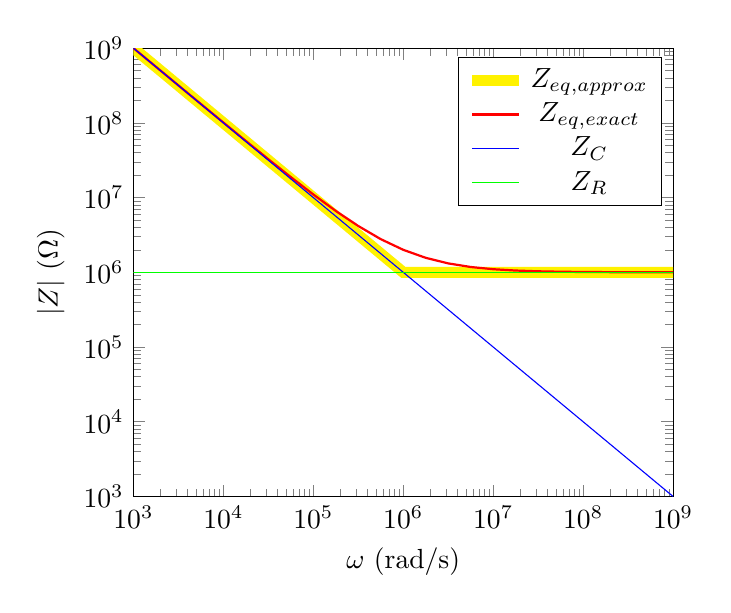
\begin{tikzpicture}
\begin{loglogaxis}[
    xlabel=$\omega$ (\SI{}{\radian / \second}), ylabel=$\abs{Z}$ (\SI{}{\ohm}),
    xmin=10^3, xmax=10^9,
    ymin=10^3, ymax=10^9,
 ]
\addplot [domain=10^3:10^9, color=yellow, line width=4pt] {max(10^12 / x, 10^6)};
\addplot [domain=10^3:10^9, color=red, thick] {10^12 / x + 10^6};
\addplot [domain=10^3:10^9, color=blue] {10^12 / x};
\addplot [domain=10^3:10^9, color=green] {10^6};
\addlegendentry{$Z_{eq, approx}$}
\addlegendentry{$Z_{eq, exact}$}
\addlegendentry{$Z_C$}
\addlegendentry{$Z_R$}
\end{loglogaxis}
\end{tikzpicture}
\end{center}
The highlighted region at the top indicates $Z_{eq, approx}$ overlapping with either $Z_C$ or $Z_R$. We see that for small values of $\omega$, the impedance of the capacitor dominates. while at high values of $\omega$, the capacitor behaves more like a short, with the resistance of the resistor dominating. Also notice that our approximation for $Z_{eq}$ is very good (on a log-log scale) at extreme values of $\omega$, and deviates most at the intersection of $Z_C$ and $Z_R$, with $\omega = \frac{1}{RC} = 10^6$ \SI{}{\radian / \sec}.

Now, we will similarly consider placing the resistor $R$ in parallel with the capacitor $C$:
\begin{center}
\begin{circuitikz}[american]
\draw (0, 0) node[circ]{} to (1, 0) to (1, 0.5) to[R, l=$R$] (3, 0.5) to (3, 0) to (4, 0) node[circ]{};
\draw (1, 0) to (1, -0.5) to[C, a=$C$] (3, -0.5) to (3, 0);
\end{circuitikz}
\end{center}
We know that the equivalent impedance magnitude can be approximated as
\[
    Z_{eq} \approx \min{(Z_R, Z_C)} = \min{(R, \frac{1}{\omega C})}.
\]
Plotting this on a log-log scale, we obtain
\begin{center}
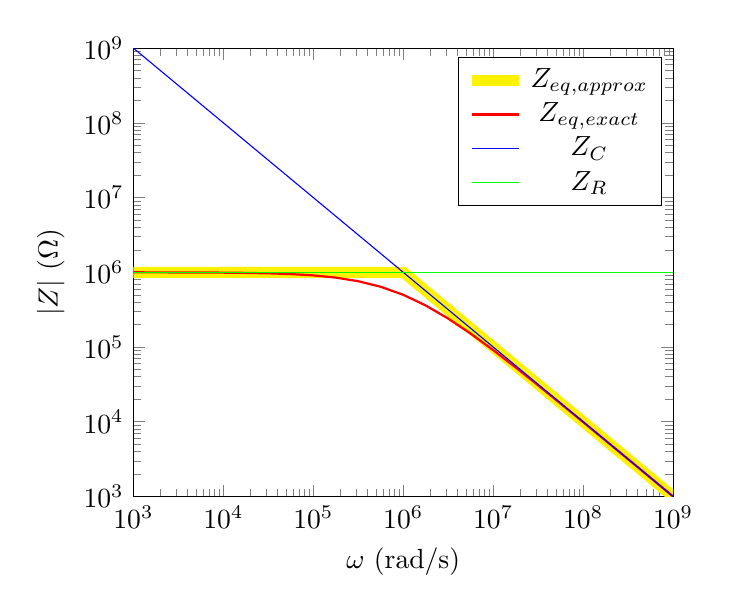
\begin{tikzpicture}
\begin{loglogaxis}[
    xlabel=$\omega$ (\SI{}{\radian / \second}), ylabel=$\abs{Z}$ (\SI{}{\ohm}),
    xmin=10^3, xmax=10^9,
    ymin=10^3, ymax=10^9,
 ]
\addplot [domain=10^3:10^9, color=yellow, line width=4pt] {min(10^12 / x, 10^6)};
\addplot [domain=10^3:10^9, color=red, thick] {1 / (x / 10^12 + 1 / 10^6)};
\addplot [domain=10^3:10^9, color=blue] {10^12 / x};
\addplot [domain=10^3:10^9, color=green] {10^6};
\addlegendentry{$Z_{eq, approx}$}
\addlegendentry{$Z_{eq, exact}$}
\addlegendentry{$Z_C$}
\addlegendentry{$Z_R$}
\end{loglogaxis}
\end{tikzpicture}
\end{center}

Here, we see that as the resistance of the capacitor is high at low frequencies, most current will flow through the resistor, meaning that $Z_R$ dominates the value of $Z_{eq}$, while at high frequencies, the capacitor behaves more like a short, so $Z_{eq}$ effectively behaves like $Z_C$. Notice also that, again, $Z_{eq, approx}$ is a good approximation for $Z_{eq}$ at extreme values of $\omega$, experiencing the largest relative error near $\omega = \frac{1}{RC} = 10^6$ \SI{}{\radian / \sec}.

It is interesting to note that varying the capacitance (or inductance) of a component only affects the y-intercept, not the slope, of its curve on a log-log scale. Thus, given two desired impedances at particular frequencies, we can construct a unique RC circuit that achieves both of them. Also note that this graphical maner of approximating equivalent impedances works just as well if an inductor replaces either the resistor or the capacitor.

\section{RC Filters}
Now, we will actually drive a voltage $V_{in}(t) = V_0\sin{\omega t}$ through a resistor and capacitor placed in series, as shown:
\begin{center}
\begin{circuitikz}[american]
\draw (0, 0) node[ocirc]{} node[left]{$V_{in}(t)$}to[R, l=$R$, i=$I$] (2, 0) to[C, l=$C$] (2, -2) node[ground]{};
\draw (2, 0) to (3, 0) node[ocirc]{} node[right]{$V_{out}$};
\end{circuitikz}
\end{center}
From our understanding of impedance, we know that
\eqn{
    && \abs{I} &= \frac{\abs{V_{in}}}{\abs{Z_{eq}}} \\
    &&&= \frac{V_0}{\max{(R, \frac{1}{\omega C})}} \\
    \thus \abs{V_{out}} &= \abs{I}Z_C \\
    &&&= \frac{V_0}{\max{(1, \omega RC)}} \\
    \thus \frac{\abs{V_{out}}}{\abs{V_{in}}} &= \frac{R}{\max{(1, \omega RC)}}.
}
The ratio of $\abs{V_{out}}$ to $\abs{V_{in}}$ is known as the \emph{transfer function}, and can be shown in most cases to be independent of the amplitude of $V_{in}$. We will first consider the case when $\omega \gg \frac{1}{RC}$, when the effects of the resistor dominate. We see here that
\[
    \frac{\abs{V_{out}}}{\abs{V_{in}}} \approx 0.
\]
Intuitively, for high frequencies the capacitor served as a short to ground, making them disappear. In contrast, for low frequencies $\omega \ll \frac{1}{RC}$, we see that
\[
    \frac{\abs{V_{out}}}{\abs{V_{in}}} \approx 1.
\]
This again makes intuitive sense, since the capacitor acts as an open circuit for low frequencies, meaning that very little current flowed across $R$, so the voltage drop from $V_{in}$ to $V_{out}$ was negligible.

Thus, this circuit is a low-pass filter. By swapping the position of the capacitor and the resistor, or by replacing the capacitor with an inductor, we can produce an analogous high-pass filter.

\section{Inductor Transients}
Finally, we will return to our previous approach of transient analysis in briefly considering the discharge of an inductor through a resistor. Recall that we showed how an inductor stores energy while current passes through it. By placing an inductor in series with a resistor, we can discharge this current, just like how a capacitor will discharge when placed in series with a resistor:
\begin{center}
\begin{circuitikz}[american]
\draw (2, 1) to[inductor, i=$I$, l=$L$] (2, -1) to (0, -1) node[ground]{} to[R, l=$R$] (0, 1) to (2, 1);
\end{circuitikz}
\end{center}

Let our initial current $I(0) = I_0$. By KVL, we have that
\eqn{
    && IR + L \frac{\dI}{\dt} &= 0 \\
    \thus IR &= -L\frac{\dI}{\dt} \\
    \thus \frac{1}{I} \dI &= -\frac{R}{L} \dt.
}
Notice that this homogenous first-order linear differential equation looks very similar to what we previously saw for capacitors. Solving in the standard manner, we find that
\[
    I(t) = I_0 e^{-\frac{R}{L}t} = I_0 e^{-t / \tau},
\]
where $\tau = \frac{L}{R}$ is the \emph{time constant} of an LR circuit. We see here that the current decreases rapidly, approaching but never quite reaching $0$, just like the behavior of the voltage across a discharging capacitor.


\end{document}
